\documentclass{article}
\usepackage{graphicx}

\begin{document}
\title{COMP6205 Web Development\\}
\author{Group 8\\Shantnu Singh - ss18g15\\Doug Morgan - dm3g14}
\date{\today}
\maketitle

\section{Overview}
    \par
        The assignment involved creating a prototype for a real-estate website aimed at university students.
        The website needs to allow: landlords to list properties, administrators to approve properties, landlords to be able to track the status of their property, and students to view approved properties.
        We have achieved all of these requirements and have added a number of other useful features, including but not limited to landlords having the ability to edit any details of a property, requiring re-approval by the University officer.

    \par
        Since the project required efficient use of ASP.NET Razor pages, a technology neither of us had used previously used, we decided to begin the project by pair programming, which allowed us to gain an understanding of how the logic of the application would work, and then develop individually later on, each of us working on a set of features.
        This meant that tasks could easily be split between us.

    \par
        To make programming separately easier, we used Git for version control.
        Visual Studio 2017 was the ideal IDE as it had in-build Razor development support, such as; IntelliSense, for code completion; package management, through NuGet and deployment to Azure.
        An SQL Express database was used and initialised through migrations created using the IDE.

\section{Design}
    \par
        Before we could start programming, some thought had to be given to the design of the user interface and database.
        We did this on pen and paper and using tools such as LucidChart.
        The logo for the website was also created at this time and other images we used were sourced from the copyright-free section of Google Images.
        The initial design of the website and the final database design is shown in Figures \ref{fig:early_sketches} and \ref{fig:sql_tables}.

        \begin{figure}[ht]
            \centering
            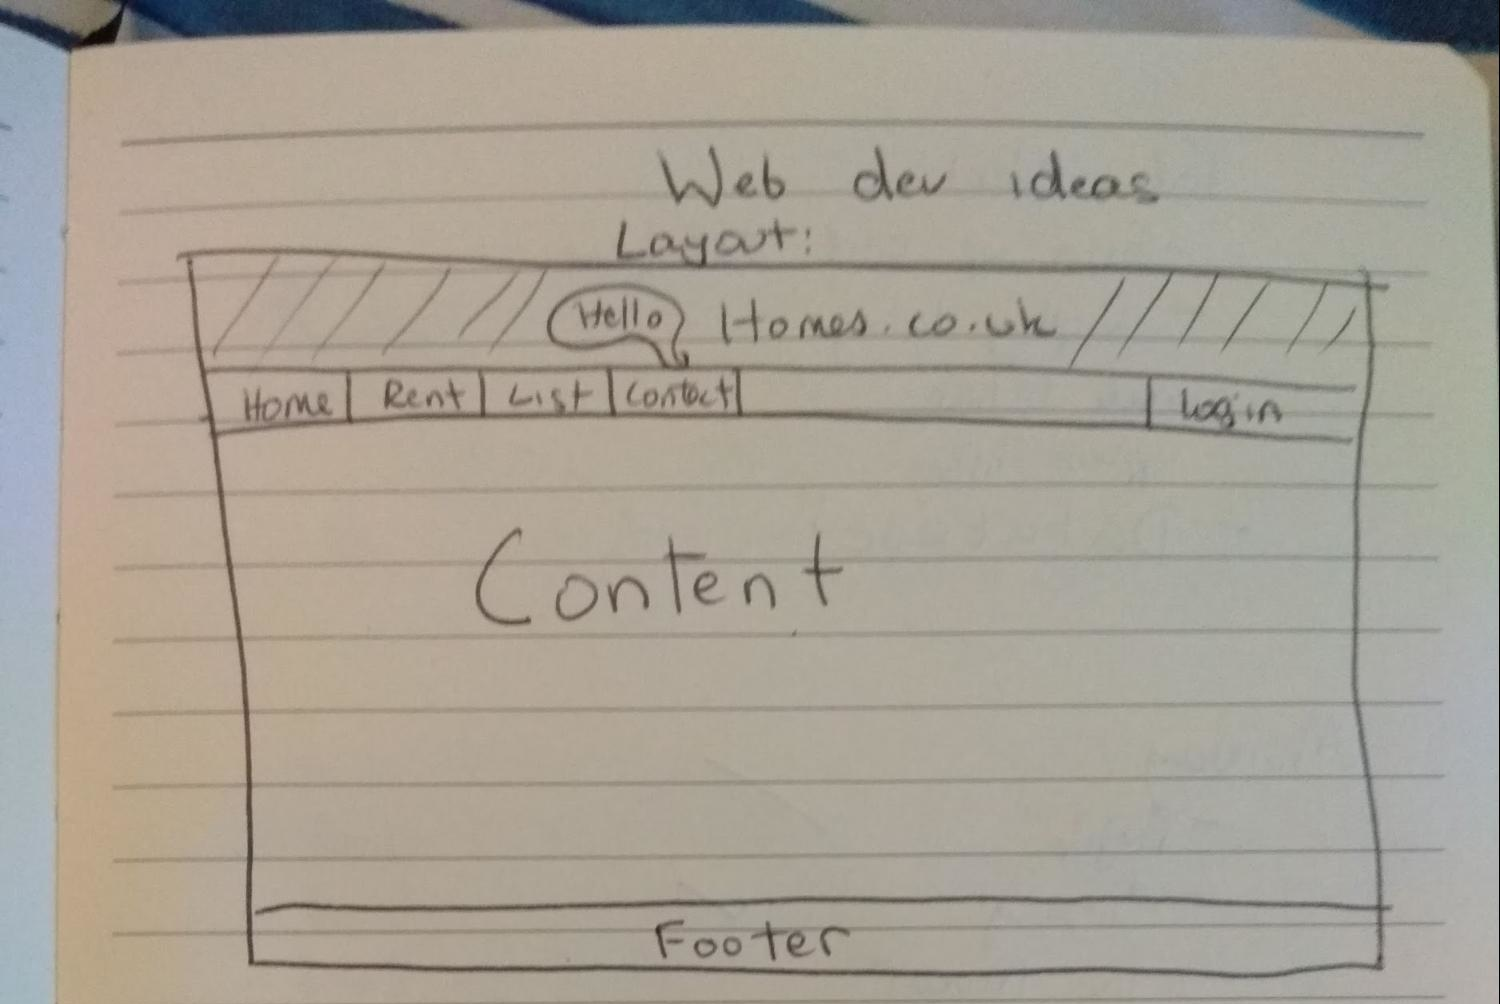
\includegraphics[width=0.48\textwidth]{figures/layout_sketch1.png}
            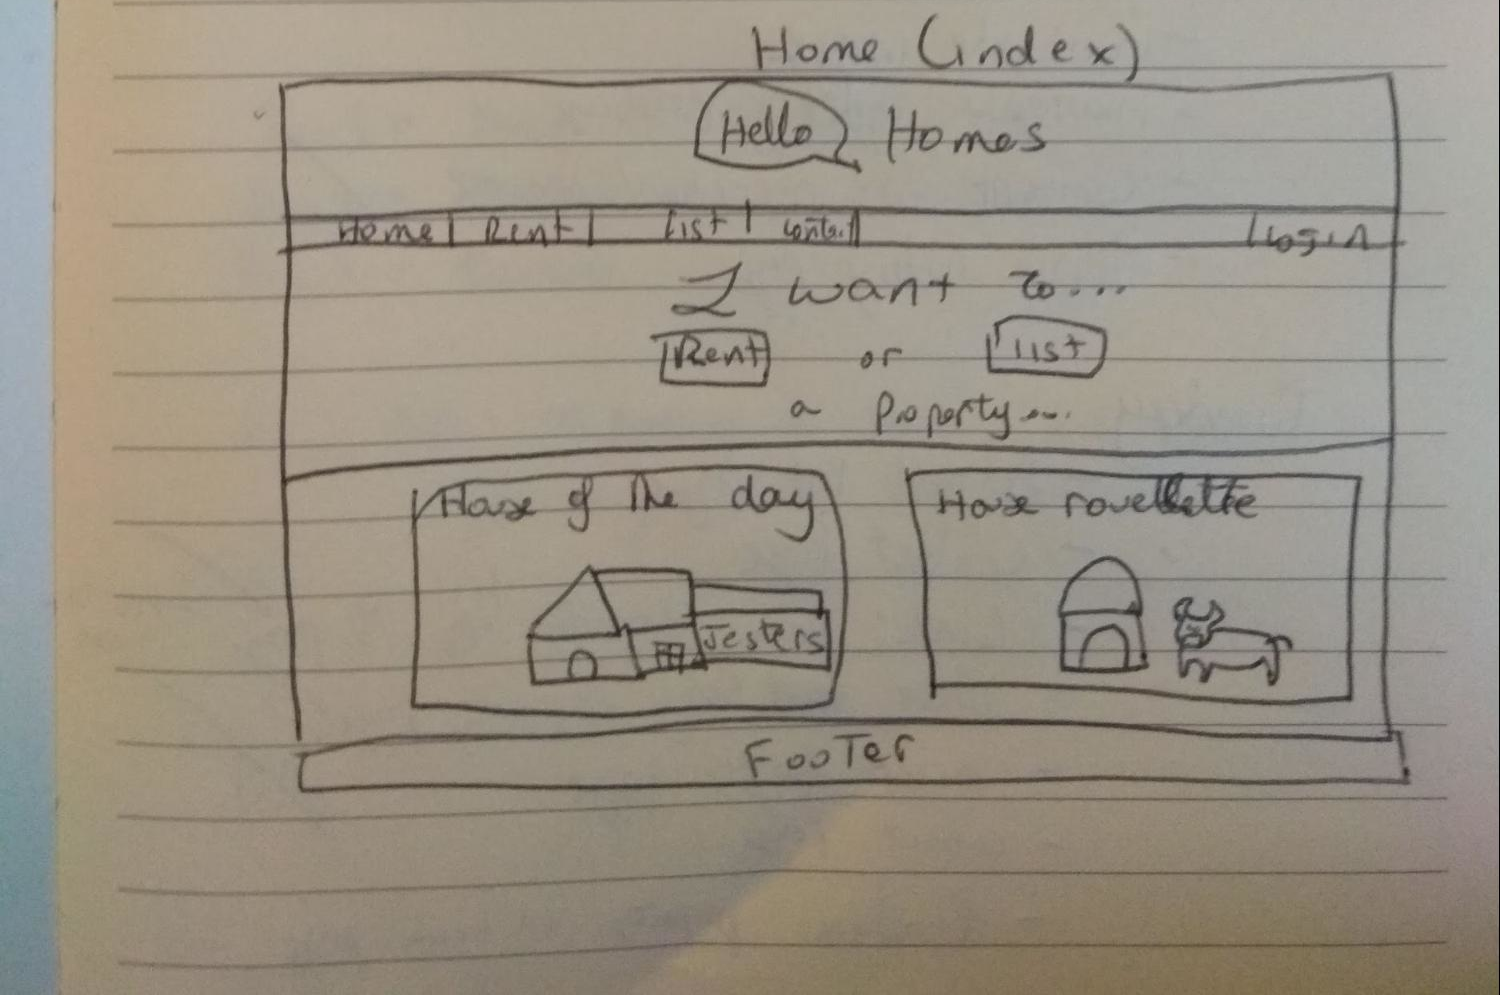
\includegraphics[width=0.48\textwidth]{figures/layout_sketch2.png}
            \caption[Early Sketches]{Early sketches of the web interface}
            \label{fig:early_sketches}
        \end{figure}

        \begin{figure}[ht]
            \centering
            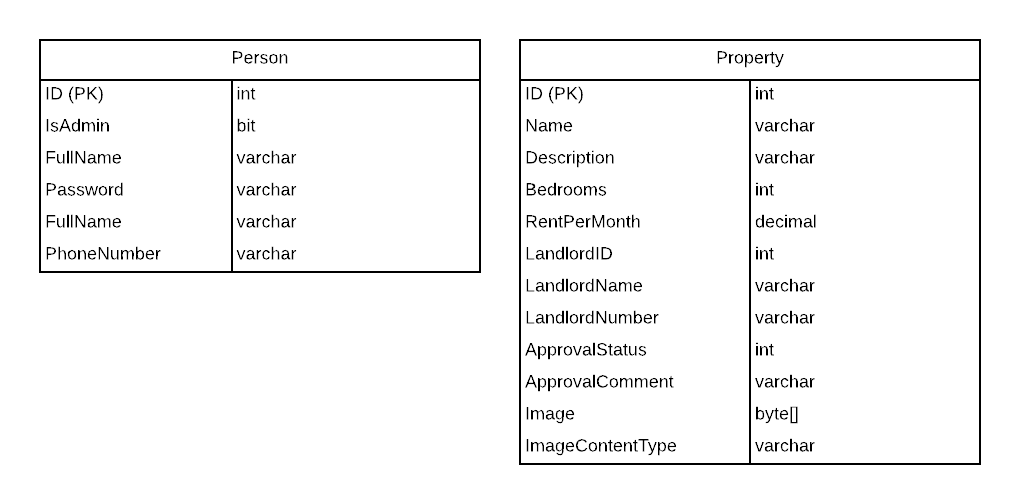
\includegraphics[width=\textwidth]{figures/sql_tables.png}
            \caption[SQL Tables]{Tables used in the final SQL database}
            \label{fig:sql_tables}
        \end{figure}

    \par
        When designing user accounts, consideration was given to all site users having an account, with different authorisation levels representing student, landlord and administrator.
        However, the student never needs to interact with the site in a way that would benefit from being logged into it, so it seemed more sensible to limit to only two kinds of user account: user and admin.
        A signed in user is able to post and edit property listings, and to see the approval status of their listings.
        An admin is able to approve or reject listings, and are required to give a brief comment in either case.
        Users who are not signed in have no capability to list properties or to view properties that have not been approved.

    \par
        The visual design has been achieved using Bootstrap, an HTML and CSS library which provides dynamically resizable elements.
        We chose this tool for greater visual consistency over manually defined parameters, as it allows portable layouts to be defined easily, so that the site can be effectively viewed on all devices.

        \begin{figure}[ht]
            \centering
            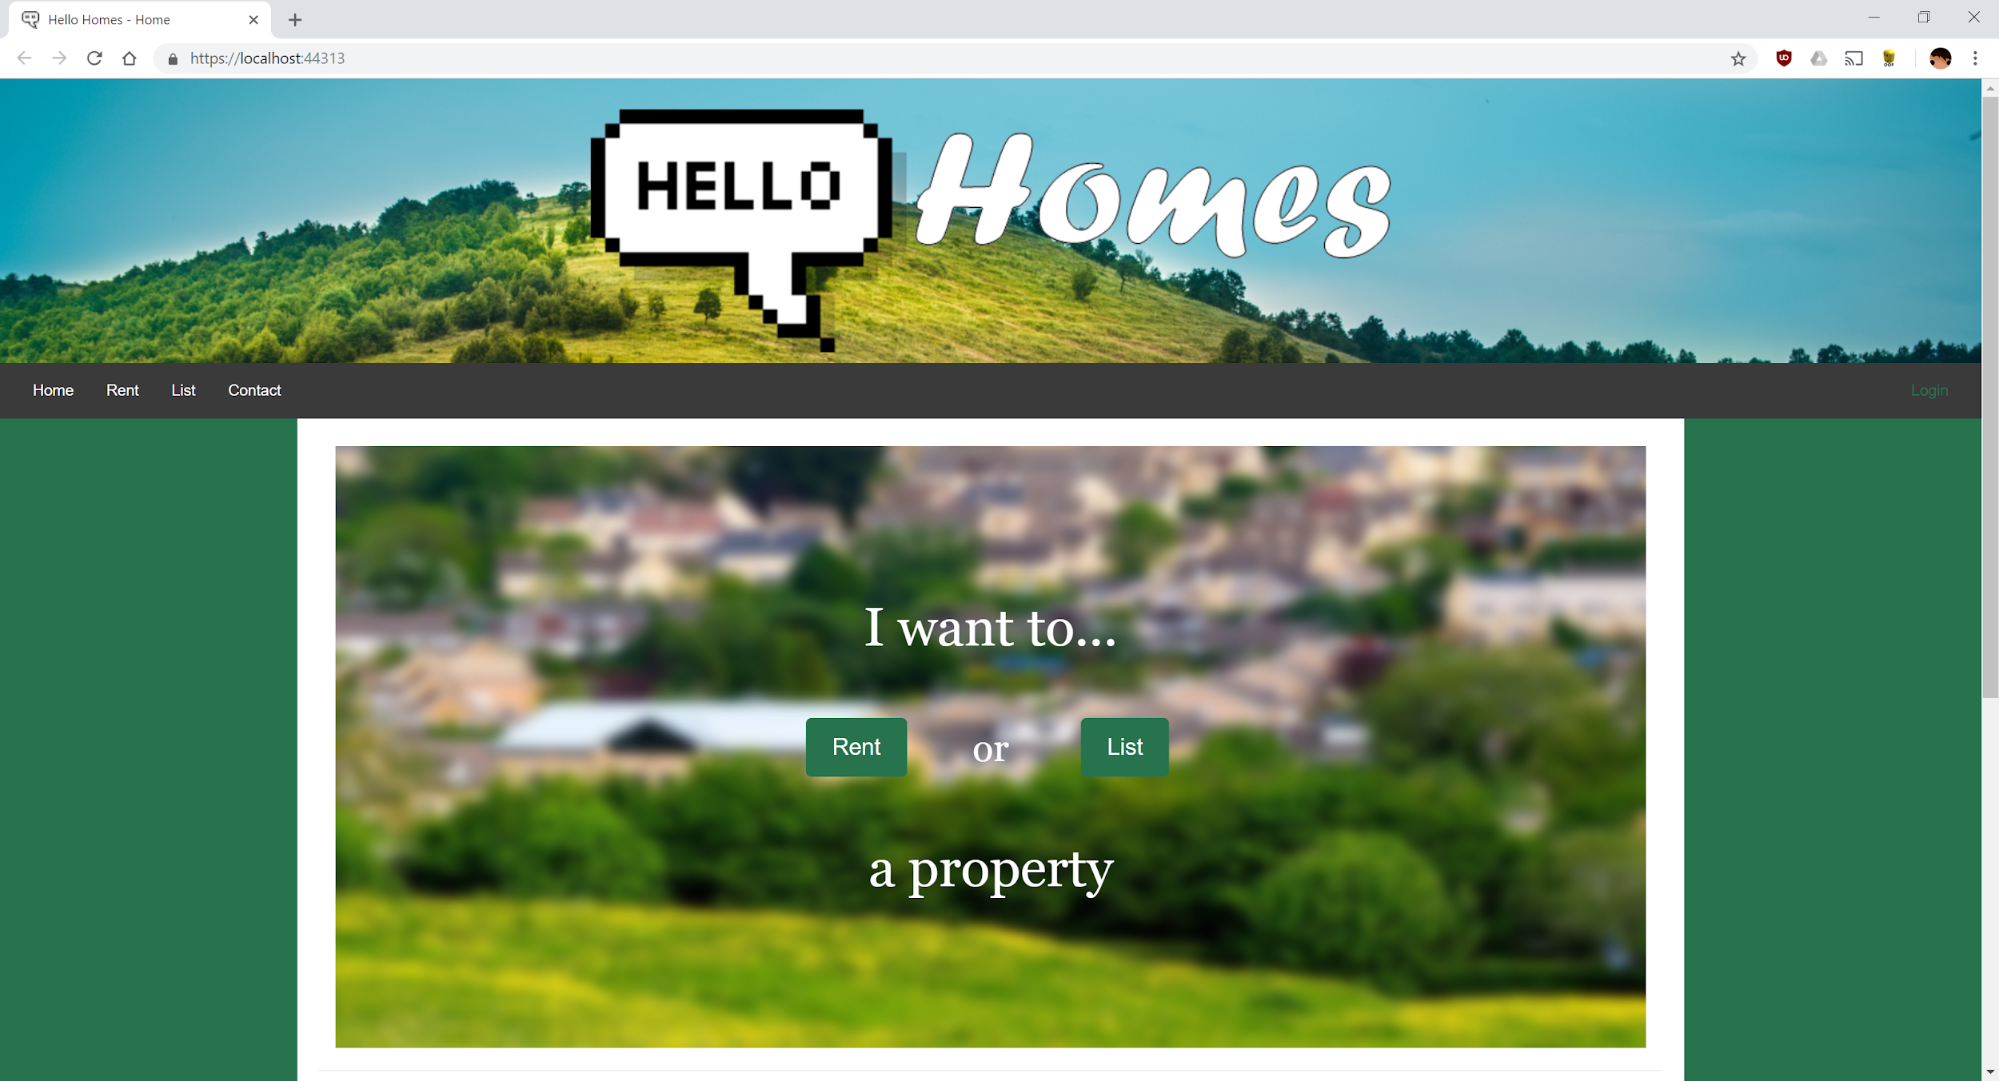
\includegraphics[width=\textwidth]{figures/index_page.png}
            \caption[Home page layout]{Layout of the home page, designed using Bootstrap}
            \label{fig:index_page}
        \end{figure}

\section{Features}
    \subsection{Main Features}

    \subsection{Additional Features}

\section{Testing}

\section{Extensions}

\section{Critical Evaluation}

\begin{thebibliography}{1}
    \bibitem{cooper88}
        Cooper, R. and Kaplan, R.S., 1988. Measure costs right: make the right decisions. Harvard business review, 66(5), pp.96-103.
\end{thebibliography}

\end{document}
